\chapter{Υλοποιήσεις}
\label{chapter:implementations}

Στο κεφάλαιο αυτό θα αναφερθούμε στις τρεις διαφορετικές εκδόσεις του συστήματος που
υλοποιήσαμε και τους λόγους που μας ώθησαν να κάνουμε αυτές τις αλλαγές.

Πριν ξεκινήσουμε, όμως, θα πρέπει να ορίσουμε τις βασικές ενέργειες που θα εκτελεί ένα τέτοιο σύστημα.
Αρχικά θέλουμε να έχει δυνατότητες server, ώστε να εξυπηρετεί απομακρυσμένους χρήστες που συνδέονται μέσω του δικτύου.
Το σύστημα επιπροσθέτως θα πρέπει να μπορεί να στέλνει αιτήματα σε εξωτερικούς servers, ιστοσελίδες και γενικά
εφαρμογές που επικοινωνούν με το διαδίκτυο. Σε αυτό το σημείο τονίζουμε την αναγκαιότητα ύπαρξης μίας βάσης δεδομένων που θα αποθηκεύει
πληροφορία σχετική με την ορθή λειτουργία του συστήματος. Τέλος και ίσως το πιο σημαντικό, απαιτείται η ύπαρξη κάποιας
μορφής scheduling, ενός μηχανισμού δηλαδή που θα ρυθμίζει πότε θα γίνονται τα αιτήματα και ποια από αυτά πρέπει γίνουν.

Όλα αυτά αφορούν αποκλειστικά τη λειτουργία του backend του συστήματος. Πέρα από αυτά
θα πρέπει να υπάρχει μία γραφική διεπαφή, μέσω της οποίας, κάθε χρήστης θα μπορεί να δει τα δεδομένα που παράγονται
από τη χρήση του συστήματός.

Πλέον και χάριν συντομίας, στο υπόλοιπο κομμάτι της διπλωματικής αυτής εργασίας, θα αναφερόμαστε
στο σύστημα που δημιουργήσαμε, με το όνομα \textbf{Lychte} (/licht/). Η ονομασία αυτή προκύπτει από τα αρχικά του "\textbf{L}ightweight
\textbf{Y}et \textbf{C}onfigura\hyp{}ble \textbf{H}ΤTP \textbf{T}raffic \textbf{E}xpert", που περιγράφει την λειτουργία και μόνο
μερικά από τα πολλά χαρακτηριστικά του συστήματος μας.

\section{Version 0.0.1}
\label{section:first_implementation}

Η πρώτη και πιο απλή έκδοση του υπό κατασκευής συστήματος Ενεργής Παρακολούθησης. Αποτελείται από έναν
nodejs server (και πιο συγκεκριμένα express server), ο οποίος είναι υπεύθυνος για τον χειρισμό όλων των λειτουργιών της εφαρμογής. Αυτός συνδέεται
άμεσα με μία MongoDB που θα αποτελέσει τη βάση δεδομένων του συστήματος.

Ο server αρχικά στεγάζει το api της εφαρμογής. Μέσα από αυτό, κάθε χρήστης που έχει πρόσβαση στο σύστημα (σωστά credentials)
μπορεί να αντλεί πληροφορία ήδη αποθηκευμένη στη βάση ή να την τροποποιεί και να δημιουργεί νέα. Τα δεδομένα που μπορεί να παράξει
είναι περιορισμένα, βέβαια, καθώς υπάρχουν collections στα οποία γράφει μόνο το ίδιο το backend. Για να συνεχίσουμε και να δούμε το υπόλοιπο σύστημα
θα πρεπει να αναφερθούμε στο pipeline της εφαρμογής, στα βήματα δηλαδή που θα ακολουθήσει ο χρήστης εντός αυτής.

Κύρια λειτουργία του Lychte είναι η αυτόματη παρακολούθηση του χρόνου λειτουργίας και απόκρισης ενός ιστοτόπου.
Για να γίνει αυτό ο χρήστης θα πρέπει να εισάγει το url, που επιθυμεί να επιβλέπει και να ενημερώνεται σχετικά με
τη κατάστασή του, και ένα χρονικό διάστημα βάσει του οποίου θα γίνονται επαναλαμβανόμενα αιτήματα.
Έπειτα η πληροφορία αυτή μεταφέρεται στον server υπό τη μορφή HTTP request. Αυτός χρησιμοποιεί το μήνυμα που έλαβε, που περιέχει το url και
όποια ακόμα πληροφορία απαιτείται (headers, body), για να κάνει μία δοκιμαστική κλήση στο σύστημα που ο χρήστης έχει επιλέξει. Αν το αίτημα εκτελεστεί επιτυχώς
το αποθηκεύει στη βάση δεδομένων και ξεκινάει έναν απλό scheduler
ο οποίος είναι υπεύθυνος για τον έλεγχου του συγκεκριμένου url.

Καταλήγουμε έτσι στη δεύτερη, μεγάλη, λειτουργία του server, το scheduling. Κάθε φορά που αποθηκεύεται ένα καινούργιο
αίτημα για παρακολούθηση, ξεκινάει μία νέα διεργασία εντός αυτής που ήδη τρέχει (αυτής του server). Η διεργασία παιδί (child process),
λαμβάνει κάποια πληροφορία, σχετικά με το αίτημα που θα πρέπει να εκτελεί, από την διεργασία που την δημιούργησε. Η τελευταία μάλιστα
έχει τη δυνατότητα να σταματήσει τη λειτουργία όσων διεργασιών έχει ξεκινήσει, αρκεί να γνωρίζει το pid που χαρακτηρίζει κάθε μία μονοσήμαντα.

\begin{figure}[!ht]
	\centering
	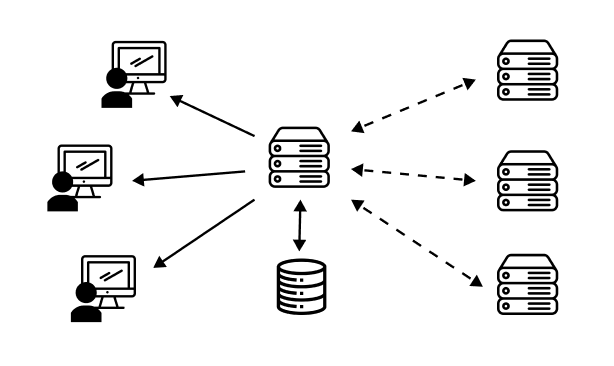
\includegraphics[width=0.8\textwidth]{./images/chapter4/lychte-first-implementation.png}
	\caption[Διάγραμμα πρώτης Υλοποίησης]{Διάγραμμα Πρώτης Υλοποίησης Συστήματος Ενεργής Παρακολούθησης. Ένας express server, με μία mongo βάση δεδομένων εξυπηρετούν χρήστες, ενώ παράλληλα στέλνουν αιτήματα σε εξωτερικά συστήματα προς παρακολούθηση}
	\label{fig:first_implementation}
\end{figure}

Όλες οι διεργασίες εκτελούν την ίδια συνάρτηση, τα ορίσματα της οποίας αποτελούν τα χαρακτηριστικά που ορίζει ο χρήστης
κατά τη διαδικασία δημιουργίας του αιτήματος προς παρακολούθηση. Η συνάρτηση αυτή είναι υπεύθυνη για να κάνει την κλήση στο εξωτερικό
σύστημα, να λάβει την απάντηση, να την αναλύσει (ανάλογα με το είδος της αναμενόμενης απάντησης) και να την αποθηκεύσει,
μαζί με κάποιες ακόμα χρήσιμες πληροφορίες, στη βάση δεδομένων. Πέρα από το response που μπορεί να είναι απλό κείμενο (html), αντικείμενο (json) ή κάποιο
αρχείο, αποθηκεύονται και οι χρονισμοί του αιτήματος, το πότε δηλαδή ξεκίνησε το αίτημα, πότε τελείωσε καθώς και το χρόνο που μεσολάβησε μεταξύ τους. Το τελευταίο
θα μπορούσε να υπολογιστεί και εκ των υστέρων σε κάθε αίτημα που το χρειάζεται, καθώς είναι δεδομένο που προκύπτει από αυτά που ήδη υπάρχουν.
Εξαιτίας όμως της φύσης του συστήματος και των δεδομένων που συλλέγονται,
θεωρούμε ότι κρίνεται αναγκαίο να κερδίσουμε επεξεργαστική ισχύ αποφεύγοντας υπολογισμούς
για δεδομένα που γνωρίζουμε ότι θα ζητούνται συνεχώς, ώστε να εξηπυρετούνται όσο το δυνατό
πιο γρήγορα και άμεσα τα αιτήματα του χρήστη ως προς τον server.

Ένα τέτοιο σύστημα μπορεί να λειτουργήσει όπως ακριβώς περιγράψαμε παραπάνω. Έχει όμως κάποια βασικά μειονεκτήματα.
Αρχικά δεν υπάρχει κάποιο κοινό σημείο αναφοράς (single point of reference). Όσες διεργασίες υπάρχουν μέσα στο server, λειτουργούν αυτόνομα,
χωρίς να υπάρχει κάποιος τρόπος να αναφερθείς σε κάποια αν δεν γνωρίζεις εκ των προτέρων το pid της και αν δεν έχεις πρόσβαση
στο σύστημα που τις εκτελεί. Επίσης, το χαρακτηριστικό αυτό των διεργασιών έχει υπόσταση μόνο εντός του ιδίου περιβάλλοντος εκτέλεσης. Ακόμα και
να αποθηκεύαμε το pid της διεργασίας που είναι υπεύθυνο για την εκτέλεση ενός συγκεκριμένου αιτήματος, δεν θα μπορούσαμε να το χρησιμοποιήσουμε
κάπως σε περίπτωση που επανεκκινηθεί το υπολογιστικό σύστημα που φιλοξενεί τον server, καθώς οι καινούργιες διεργασίες θα είχαν διαφορετικό id.
Οι "καινούργιες διεργασίες" εδώ χαρακτηρίζουν ένα σύνολο διεργασιών που θα ξεκινούσε ο server μέχρι όλα τα αιτήματα που βρίσκονται αποθηκευμένα στη βάση
να ξεκινήσουν να ελέγχονται από κάποιο process.

Αξίζει ακόμα να σημειωθεί ότι το σύστημα αυτό δεν μπορεί να κλιμακωθεί εύκολα και αποδοτικά, καθώς
για να επεκταθεί το σύνολο των αιτημάτων που διαχειρίζονται, θα πρέπει να προστεθεί κι ένας δεύτερος server, που ίσως δεν χρειάζεται να επιτελεί κάποια λειτουργία,
ώστε να χωρέσουν παραπάνω διεργασίες. Το πρόβλημα αυτό όμως μπορεί να λυθεί σπάζοντας τις δύο βασικές λειτουργίες του
Lychte σε δύο διακριτές και σαφώς ανεξάρτητες οντότητες, ενός scheduler και ενός server. Αυτό ακριβώς θα μελετήσουμε και στην επόμενη υλοποίηση του συστήματός μας.

\newpage

\section{Version 0.1.0}
\label{section:second_implementation}

Συνεχίζοντας τη συλλογιστική πορεία της πρώτης υλοποίησης, καλούμαστε να λύσουμε ένα από τα πιο βασικά προβλήματα που προέκυψαν,
τον διαμοιρασμό των λειτουργιών. Όπως προαναφέραμε θα πρέπει να υπάρχει ένας server που θα εξυπηρετεί
τους χρήστες μέσω των προγραμματιστικών διεπαφών που παρέχει, και ένας ή παραπάνω schedulers, που θα εκτελούν
αποκλειστικά και μόνο αιτήματα προς τα συστήματα που θέλουμε να ελέγχουμε. Ας δούμε όμως πιο συγκεκριμένα το ανανεωμένο σύστημα (\autoref{fig:second_implementaion})

\begin{figure}[!ht]
	\centering
	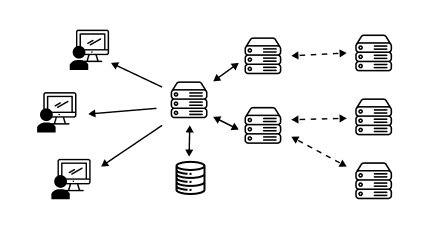
\includegraphics[width=0.8\textwidth]{./images/chapter4/lychte-second-implementation.png}
	\caption[Διάγραμμα δεύτερης Υλοποίησης]{Διάγραμμα Δεύτερης Υλοποίησης Συστήματος Ενεργής Παρακολούθησης. Αποτελείται στο κέντρο του από έναν express server και μία mongo βάση δεδομένων. Ο server επικοινωνεί με δύο schedulers οι οποίοι είναι υπεύθυνοι για τον έλεγχο εξωτερικών προς το σύστημα εφαρμογών/server}
	\label{fig:second_implementaion}
\end{figure}

Το βασικό συστατικό του Lychte, ο server δηλαδή παραμένει όπως είχε. Έχει δηλαδή routes μέσα από τα οποία εξυπηρετεί τα αιτήματα
των χρηστών που προέρχονται από το frontend του συστήματος. Αυτά αφορούν την αποστολή πληροφορίας προς τους χρήστες προκειμένου να δουν
τα δεδομένα που αποθηκεύουμε στη βάση μας, αλλά και την αποθήκευση πληροφορίας που προέρχεται από τους χρήστες που σχετίζεται με τη δημιουργία
καινούργιων ελέγχων σε urls που επιθυμούν να παρακολουθούν.

Αυτό που αλλάζει σε σχέση με την προηγούμενη υλοποίηση, είναι ο τρόπος που διευθετεί
την εκτέλεση των επαναλαμβανόμενων αιτημάτων που πρέπει να κάνει προς τα εξωτερικά υπό παρακολούθηση συστήματα.
Όπως είπαμε νωρίτερα, δεν είναι πλέον υπεύθυνος για το scheduling των ενεργειών που πρέπει να γίνουν,
αλλά αντιθέτως στέλνει σε ένα άλλο σύστημα (scheduler) τις πληροφορίες που χρειάζεται προκειμένου να ρυθμιστεί και να οργανωθεί κατάλληλα
ο έλεγχος των urls που θέλουμε να ελέγχονται.

Πλέον θα αναφερόμαστε στο σύστημα του scheduler ως worker, καθώς αυτό που κάνει είναι να λαμβάνει δεδομένα και να
εκτελεί, βάσει αυτών, συνεχώς αιτήματα προς άλλα εξωτερικά συστήματα. Ο τρόπος λειτουργίας του είναι αρκετά παρόμοιος
με αυτή του scheduler της πρώτης υλοποίησης, με κάποιες μικρές διαφορές. Κάθε φορά που λαμβάνει κάποιο αίτημα από τον κεντρικό server, κάνει ένα δοκιμαστικό request
στο url που πρόκειται να ελεγχθεί, για να διαπιστωθεί η ορθότητά του. Έπειτα ξεκινάει έναν timer που εκτελεί το αίτημα στα χρονικά διαστήματα που ορίζει ο χρήστης. Ο χρόνος αυτός θα μπορούσε να φτάνει μέχρι και το ένα δευτερόλεπτο, αλλά για λόγους σταθερότητας και
εγγύησης ότι η εκτέλεση κάποιου αιτήματος δεν θα μπλοκάρει την εκτέλεση κάποιου άλλου, έχουμε βάλει ένα κάτω όριο των 30 δευτερολέπτων στην υλοποίησή μας.
Στην περίπτωση που το αίτημα χρειαστεί χρόνο, για να ικανοποιηθεί, μεγαλύτερο αυτού που έχει οριστεί σαν χρόνος μεταξύ
διαδοχικών αιτημάτων διακόπτουμε το αίτημα μέσω timeouts και το αποθηκεύουμε στη βάση σαν αποτυχημένη απόκριση (failed response).
Αυτό γίνεται για να εξασφαλίσουμε ότι το χρονικό διάστημα μεταξύ διαδοχικών αιτημάτων θα παραμένει
σχετικά σταθερό και η απόλυτη μετατόπιση του χρόνου που υπάρχει μεταξύ των αιτημάτων σε βάθος χρόνου,
δεν θα αλλάζει σε μεγάλο βαθμό.

Για να γίνει πιο κατανοητό το παραπάνω αρκεί να μελετήσουμε τα \cref{fig:perfect_request_cycle,fig:timeouts_request_cycle}.

Το πρώτο περιγράφει την εκτέλεση ενός αιτήματος σε χρονικό διάστημα ενός λεπτού. Όπως παρατηρούμε το
αίτημα εκτελείται επιτυχώς σε αυτό το μήκος χρόνου, με αποτέλεσμα, όταν έρθει η στιγμή που πρέπει να επαναεκτελεστεί,
αυτό να γίνει χωρίς περιττές καθυστερήσεις. Αν υποθέσουμε ότι ο χρόνος που μεσολάβησε, μεταξύ του πρώτου και του δεύτερου αιτήματος,
είναι ακριβώς εξήντα δευτερόλεπτα, μπορούμε να πούμε ότι η απόκλιση μεταξύ αυτών είναι μηδενική.
Βέβαια κάτι τέτοιο δεν υφίσταται στην πραγματικότητα καθώς οι timers έχουν πάντα μία μικρή απόκλιση, προς τα πάνω ή προς τα κάτω, της τάξης των nanoseconds.
Σε βάθος χρόνου η απόκλιση παραμένει κοντά στο μηδέν.

\begin{figure}[!ht]
	\centering
	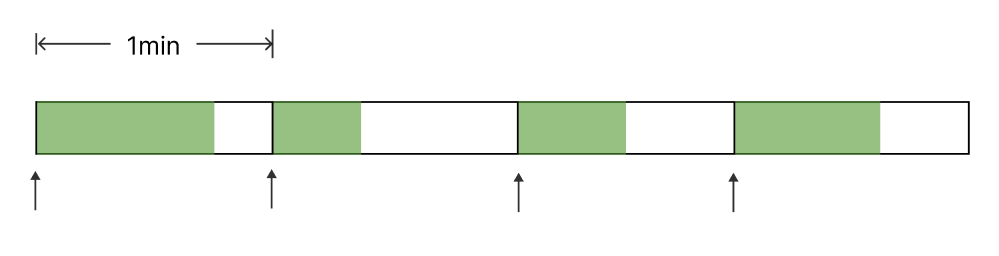
\includegraphics[width=0.8\textwidth]{./images/chapter4/perfect_request_cycle.png}
	\caption[Κύκλος Ζωής εκτέλεσης ενός επαναλαμβανόμενου Αιτήματος]{Κύκλος Ζωής εκτέλεσης ενός επαναλαμβανόμενου Αιτήματος}
	\label{fig:perfect_request_cycle}
\end{figure}

Έπειτα ας μελετήσουμε την περίπτωση που το αίτημα χρειάζεται παραπάνω χρόνο για να εκτελεστεί (εξαιτίας καθυστερήσεων του εξωτερικού συστήματος που ελέγχεται).
Στο \autoref{fig:timeouts_request_cycle} μπορούμε να δούμε ακριβώς πως θα λειτουργούσε ένας worker στην περίπτωση που υπήρχαν μεγάλες εξωγενείς καθυστερήσεις, χωρίς τη χρήση
timeous αλλά και με τη χρήση αυτών. Όταν αναφερόμαστε σε timeouts περιγράφουμε την πρόωρη έξοδο από τη συνάρτηση που τρέχουμε, στην
προκειμένη την εκτέλεση του αιτήματος. Παρατηρούμε ότι στα δύο χρονικά διαγράμματα έχουμε αρκετά μεγάλες διαφορές.
Στο πρώτο περιμένουμε να εκτελεστεί πλήρως το αίτημα, ακόμα και αν αυτό αργήσει παραπάνω από όσο
θα έπρεπε. Το επόμενο αίτημα ξεκινάει με κάποια καθυστέρηση ως προς το πρώτο και παρομοίως τα επόμενα στη σειρά.
Αυτή η διαδικασία εισάγει απόκλιση στους χρόνους των κλήσεων μεταξύ των αιτημάτων που υπό φυσιολογικές συνθήκες αναμένουμε να ισαπέχουν (χρονικά) μεταξύ τους.
Απόκλιση η οποία μάλιστα μπορεί συνεχώς να αυξάνεται, καθιστώντας το σύστημά μας αναξιόπιστο ως προς
το χρόνο εκτέλεσης και την ακρίβεια των αιτημάτων. Για αυτό το λόγο κρίνουμε αναγκαία τη χρήση timeouts.
Το μεινέκτημα σε αυτή την περίπτωση είναι ότι αποθηκεύουμε ως εσφαλμένο ένα πιθανώς σωστό response, λόγω του χρόνου που πήρε για να εκτελεστεί.

\begin{figure}[!ht]
	\centering
	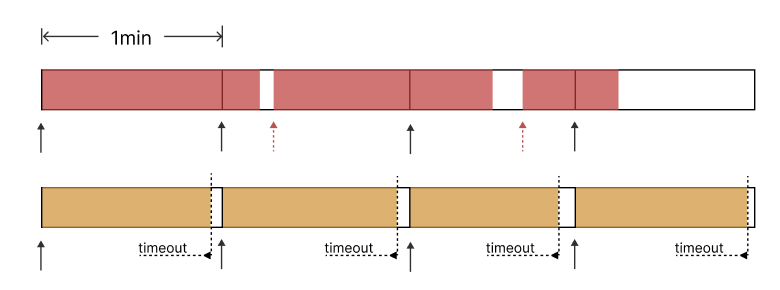
\includegraphics[width=0.8\textwidth]{./images/chapter4/timeout_request_cycle.png}
	\caption[Σύγκριση χρήσης ή μη timeouts στον κύκλο ζωής εκτέλεσης ενός αργού επαναλαμβανόμενου αιτήματος]{Σύγκριση χρήσης ή μη timeouts στον κύκλο ζωής εκτέλεσης ενός αργού επαναλαμβανόμενου αιτήματος}
	\label{fig:timeouts_request_cycle}
\end{figure}

Μία ακόμα αλλαγή ως προς την πρώτη υλοποίηση αφορά την επικοινωνία μεταξύ server και worker. Προκειμένου το σύστημα να
μπορεί να σπάσει σε πιο διακριτές έννοιες, χάνουμε το πλεονέκτημα του να έχουμε όλες τις λειτουργίες εντός του ίδιου συστήματος.
Οι λειτουργίες, όμως, αυτές, για να επιτελούνται, πρέπει να υπάρχει ένα τρόπος επικοινωνίας μεταξύ των εμπλεκόμενων.
Η επικοινωνία αυτή δεν θα είναι απαραίτητα μονόπλευρη. Η βασική λειτουργία, όπως είχαμε δει και από την προηγούμενη υλοποίηση,
είναι η αποστολή μηνυμάτων στον scheduler, σε αυτή την περίπτωση στον worker. Επεκτείνοντας όμως τις δυνατότητες του συστήματος
θα μπορούσαμε να έχουμε αμφίδρομη επικοινωνία μεταξύ server και worker, ώστε να μπορεί να ενημερώνεται ο server (όταν το ζητήσει) για την
κατάσταση των διάφορων workers που είναι συνδεμένοι σε αυτόν. Κάτι τέτοιο θα είχε νόημα αν είχαμε παραπάνω από έναν worker και θα θέλαμε να κάνουμε
διαμοιρασμό φόρτου σε καθέναν από αυτούς. Αρχικά ο server, θα ρωτούσε όλους τους συνδεδεμένους workers σχετικά με το πλήθος των αιτημάτων
που ελέγχουν τη δεδομένη χρονική στιγμή. Έπειτα κάθε κόμβος θα απαντούσε, και αυτός με το λιγότερο φόρτο θα επιλεγόταν ως ο κατάλληλος
για τη δημιουργία μίας ακόμα διεργασίας ελέγχου ενός url.

Λόγω της αμφίδρομης σχέσης που έχουν τα δύο συστήματα μεταξύ τους, επιλέχθηκε το πρωτόκολλο επικοινωνίας των WebSockets.
Πιο συγκεκριμένα ο τρόπος ενσωμάτωσης της τεχνολογίας αυτής πραγματοποιήθηκε με τη χρήση της βιβλιοθήκης \textbf{socket.io} που αποτελεί ένα
abstract layer πάνω από το πρωτόκολλο WebSockets. Για να υπάρξει επικοινωνία θα πρέπει να υπάρχει από τη μία πλευρά ένας \textbf{socket.io-server} και από την άλλη, ένας \textbf{socket.io-client}.
Στη δική μας εφαρμογή, ο socket.io-server θα είναι ο server και ο socket.io-client οι workers. Κάθε φορά που θα ξεκινάει τη λειτουργία του ένας server, θα δημιουργεί στο τοπικό δίκτυο του
έναν socket server στον οποίο μπορούν να συνδεθούν και να επικοινωνήσουν όσοι διαθέτουν το url του και τα απαραίτητα credentials. Από την άλλη,
κάθε φορά που ξεκινάει τη λειτουργία του ένας worker, θα πρέπει να μπορεί να συνδέεται κατευθείαν στοv socket server που υπάρχει.
Θα πρέπει δηλαδή να διαθέτει από πριν το url που οδηγεί στον socket server.

Οι λόγοι που επιλέχθηκαν τα WebSockets αντί ενός κλασσικού HTTP server είναι κυρίως οι ταχύτητες που προσφέρουν και η αμφίδρομη επκοινωνία. Υπό περιτπώσεις
μπορεί να είναι μέχρι και δέκα φορές πιο γρήγορα σε σχέση με το συμβατικό πρωτόκολλο HTTP. Επίσης από τη στιγμή που κάθε worker
θα επικοινωνεί αποκλειστικά με έναν server του δικού μας κλειστού συστήματος βλέπουμε ότι δεν έχει νόημα η δημιουργία ολόκληρου HTTP server στο πλαίσιο λειτουργίας ενός worker.

\begin{figure}[!ht]
	\centering
	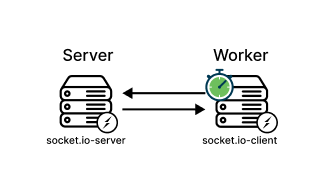
\includegraphics[width=0.8\textwidth]{./images/chapter4/socket.io-communication.png}
	\caption[Επικοινωνία server-worker μέσω websockets]{Επικοινωνία server-worker μέσω websockets}
	\label{fig:socketio-communitation}
\end{figure}

Η παραπάνω υλοποίηση έχει πολλά πλεονεκτήματα σε σχέση με την πρώτη. Αρχικά με τον καταμερισμό
των δύο βασικών λειτουργιών μειώνουμε την πολυπλοκότητα του συστήματος, κάτι το οποίο θα πρέπει να μας απασχολεί,
καθώς όσο πιο πολύπλοκο είναι ένα σύστημα τόσο πιο δύσκολα συντηρείται στη συνέχεια. Πέρα από αυτό, που αφορά
κυρίως τη διαδικασία ανάπτυξης λογισμικού και δεν επιφέρει κάποιο άμεσο κέρδος στους χρήστες, θα πρέπει να αναφέρουμε
ότι το σύστημα γενικά είναι πιο αποδοτικό, καθώς οι διεργασίες που κάθε worker στεγάζει είναι λιγότερο πιθανό να
κολλήσουν και να μπλοκάρουν λόγω φόρτου στο μηχάνημα που εκτελούνται. Τα requests γενικά δεν καταναλώνουν πολλούς πόρους από το σύστημα στο οποίο εκτελούνται,
σε αντίθεση με έναν server που μπορεί να δέχεται συνεχώς αιτήματα. Αξίζει να σημειωθεί ότι το api που παρέχει ο server του συστήματός μας είναι υπεύθυνο
για την αποστολή μεγάλου όγκου πληροφορίας, διαρκώς, που χρησιμοποιείται σε πληθώρα διαγραμμάτων, καθιστώντας τον έτσι απαιτητικό ως προς τους πόρους του
υπολογιστικού συστήματος.

Ένας ακόμα τομέας στον οποίο συνεισφέρει σε μεγάλο βαθμό η διάσπαση των λειτουργιών αφορά την κλιμάκωση, και βασικά την οριζόντια κλιμάκωση
του συστήματος. Αν δούμε ότι ο server υστερεί και δυσκολεύεται να ανταπεξέλθει στα αιτήματα των χρηστών,
μπορούμε να φτιάξουμε έναν καινούργιο server. Από την άλλη, αν παρατηρήσουμε ότι οι workers αργούν ή έχουν υπερφορτωθεί
μπορούμε να δημιουργήσουμε νέους workers και να διαμοιράσουμε τα αιτήματα εξίσου στο πλήθος των ενεργών schedulers που διαθέτουμε.

Ακόμα και με αυτή την υλοποίηση, όμως, υπάρχει έλλειψη ενός κοινού σημείου αναφοράς. Ενός κόμβου στο σύστημά μας του οποίου
οι αλλαγές θα επηρέαζαν άμεσα τη λειτουργία όλων των οντοτήτων αυτού.

\section{Version 1.0.0}
\label{section:third_implementation}

Τέλος, φτάνουμε στην τωρινή υλοποίησής μας, στην τελική πλέον έκδοση του Lychte. Πολλές ιδέες από προηγούμενες υλοποιήσεις
παρέμειναν, ελαφρώς πάντοτε τροποποιημένες με σκοπό τη βελτίωση του συστήματος. Στο \autoref{fig:third_implementation} μπορούμε να δούμε με μία πρώτη ματιά
το διάγραμμα του συστήματος

\begin{figure}[!ht]
	\centering
	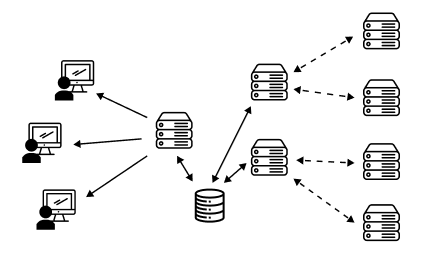
\includegraphics[width=0.8\textwidth]{./images/chapter4/lychte-third-implementation.png}
	\caption[Διάγραμμα Τελικής Υλοποίησης]{Ο server και κάθε worker του συστήματος συνδέονται με τη βάση χωρίς να υπάρχει άμεση επικοινωνία μεταξύ τους. Ο server εξυπηρετεί αποκλειστικά χρήστες, ενώ οι workers είναι υπεύθυνοι για την αποστολή αιτημάτων στα εξωτερικά συστήματα που θέλουμε να ελέγχουμε}
	\label{fig:third_implementation}
\end{figure}

Το τελικό σύστημα μοιάζει σε μεγάλο βαθμό με την προηγούμενη υλοποίηση. Η αρχιτεκτονική του server είναι σχεδόν ίδια χωρίς το κομμάτι των websockets.
Πλέον δεν υπάρχει άμεση επικοινωνία μεταξύ server και workers. Αν κάποια από τις δύο οντότητες πρέπει να μεταφέρει
πληροφορία στην άλλη, θα το κάνει γράφοντας σε κατάλληλα πεδία και συλλογές αντικειμένων ή διαγράφοντας πληροφορία εντός της βάσης δεδομένων.
Ο τύπος της βάσης εξακολουθεί να είναι noSQL και συγκεκριμένα MongoDB, λόγω της ικανότητάς της να αποθηκεύει μεγάλο πλήθος δεδομένων. Δεδομένων μάλιστα που δεν χρειάζεται
να ακολουθούν ένα συγκεκριμένο τύπο σχήματος (schema). Πέρα από αυτά οι δυνατότητες που παρέχει για sharding καθώς και για
εύκολη και γρήγορη κλιμάκωση την καθιστούν ιδανική για το σύστημα μας, που συνεχώς αποθηκεύει νέα πληροφορία στη βάση.

Πριν συνεχίσουμε στην επεξήγηση της ακριβής λειτουργίας του ανανεωμένου συστήματος, θα πρέπει να αναφερθούμε στους workers/schedulers. Η λειτουργία τους
έχει εξελιχθεί σε σχέση με τις προηγούμενες εκδόσεις. Έχοντας πλέον ένα κοινό σημείο αναφοράς, τη Mongo βάση, μπορούμε να φτιάξουμε πιο "έξυπνους" schedulers.
Στις άλλες υλοποιήσεις μας κάθε φορά που ερχόταν ένα νέο αίτημα (ένα νέο url που θα πρέπει να ελέγχουμε δήλαδή), η διαδικασία που ακολουθούσαμε ήταν απλή. Ξεκινούσαμε ένα child process
που εκτελούσε συνέχεια, ανά χρονικά διαστήματα που όριζε ο χρήστης, ένα αίτημα σε κάποιο εξωτερικό σύστημα. Όταν ο χρήστης επέλεγε να σταματήσει να
παρακολουθεί το συγκεκριμένο url, τερματίζαμε το process που έτρεχε τον έλεγχο, καθώς γνωρίζαμε από πριν το pid της διεργασίας.
Η παραπάνω διαδικασία δουλεύει καλά σε μικρό πλήθος αιτημάτων. Το πρόβλημα που δημιουργείται είναι ότι φτάνει γρήγορα σε σημείο κορεσμού, στο σημείο εκείνο που οι αποκλίσεις από τους αναμενόμενους
χρόνους μεταξύ των διαδοχικών αιτημάτων αυξάνεται συνεχώς.

Η νέα εκδοχή των workers στηρίζεται στην ύπαρξη ενός κύριου
scheduler που τρέχει κάθε n δευτερόλεπτα και ψάχνει από τη βάση ποια αιτήματα πρέπει να εκτελεστούν. Πιο συγκεκριμένα, κάθε φορά που αποθηκεύουμε ένα αίτημα προς έλεγχο στη βάση,
δημιουργούμε ένα ακόμα αντικείμενο που αφορά ένα job. Σε αυτό το αντικείμενο αποθηκεύονται πληροφορίες σχετικά με το αίτημα το οποίο θα πρέπει να εκτελείται, η ημερομηνία που
αυτό αποθηκεύτηκε, το χρονικό διάστημα μεταξύ των διαδοχικών αιτημάτων, το πότε πρέπει να εκτελεστεί ξανά το job (χρόνος δημιουργίας + χρονικό διάστημα μεταξύ αιτημάτων),
καθώς και κάποια άλλα πεδία που θα εξηγήσουμε στη συνέχεια. Κάθε τέτοιο αντικείμενο αποθηκεύεται σε μία συλλογή αντικειμένων (collection) στην οποία έχει πρόσβαση μόνο ένας
worker. Όταν εκτελούμε τον κώδικα ενός worker αρχικά ξεκινάει ένας scheduler που εκτελεί μία διεργασία κάθε δέκα δευτερόλεπτα. Η λειτουργία αυτής είναι να ψάχνει στη βάση,
και συγκεκριμένα στο collection απο το οποίο διαβάζει αποκλειστικά ο συγκεκριμένος worker, προκειμένου να βρει jobs που πρέπει να εκτελέστουν. Αν εντοπιστεί κάποιο του οποίου ο αποθηκευμένος χρόνος, που πρέπει να ξαναεκτελεστεί,
έχει ξεπεραστεί χρονικά, σημαίνει ότι πρέπει να εκτελέσει το αίτημα, τα χαρακτηριστικά του οποίου έχει αποθηκευμένα.
Αν κριθεί ότι ένα job πρέπει να ξεκινήσει να εκτελείται, τροποποιούμε στην καταχώρηση του στη βάση, ένα πεδίο (locked) που καθορίζει αν το job ήδη τρέχει ή όχι. Στην περίπτωση που αυτό είναι κλειδωμένο, κανένας scheduler
δεν θα εκτελέσει το job μέχρι να "ξεκλειδωθεί" και φυσικά να καλυφθεί η πρώτη συνθήκη σχετικά με το χρόνο πλήρωσης και τελευταίας εκτέλεσης του job.

Αξίζει σε αυτό το σημεία να σημειωθεί ότι κάθε worker θα πρέπει να διαθέτει ένα ξεχωριστό όνομα.
Αυτό γίνεται γιατί κάθε ένας διαθέτει το δικό του collection στη βάση από το οποίο διαβάζει όλα τα jobs
και μετέπειτα αποφασίζει ποια από αυτά θα τρέξουν και πότε.

\begin{figure}[!ht]
	\centering
	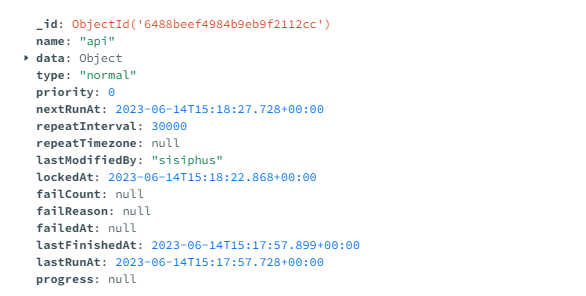
\includegraphics[width=0.8\textwidth]{./images/chapter4/sample_job_document.png}
	\caption[Παράδειγμα εγγραφής ενός \textbf{Job} στη βάση]{Παράδειγμα εγγραφής ενός \textbf{Job} στη βάση. Tο πεδίο \textit{lockedAt} έχει τιμή διάφορη του null, όταν το job ήδη εκτελείται.
		Το πεδίο \textit{nextRunAt} υπολογίζεται από το άθροισμα του χρόνου πλήρωσης της προηγούμενης εκτέλεσής του (\textit{lastFinishedAt}) και του interval. Στο πεδίο \textit{data}
		έχει αποθηκευμένη όλη την πληροφορία που χρειάζεται για να εκτελέσει το αίτημα για το οποίο δημιουργήθηκε το συγκεκριμένο job. Βάσει των πεδίων αυτών κυρίως κρίνεται το αν ο
		κεντρικός scheduler θα ξεκινήσει τη διεργασία}
	\label{fig:sample_job_document}
\end{figure}

Στη συνέχεια θα δούμε την πορεία της πληροφορίας στο σύστημα που υλοποιήσαμε.

\begin{enumerate}
	\item Ο χρήστης εισάγει κάποιο url το οποίο επιθυμεί να ελέγχεται ανά κάποιο συγκεκριμένο χρονικό διάστημα.
		Πέρα από την εισαγωγή της διεύθυνσης της ιστοσελίδας έχει τη δυνατότητα να παραμετροποιεί το αίτημά που θα
		εκτελείται επιλέγοντας headers, body (σε περίπτωση post αιτήματος), query, μέθοδο HTTP (get, put, post, delete) και τύπο απόκρισης (json, text, stream).
		Επιπλέον μπορεί να επιλέγει το πόσο συχνά θα γίνονται οι διαδοχικοί έλεγχοι.
		Πιο συγκεκριμένα, μπορεί να επιλέξει χρονικά διαστήματα από τριάντα δευτερόλεπτα μέχρι και διάστημα μία ολόκληρης ημέρας.
		Τέλος, στο κομμάτι της παραμετροποίησης μπορεί να καθορίσει την επιθυμητή κατάσταση απόκρισης του αιτήματος (εξ ορισμού \textbf{Status Code 200}) και ένα response body,
		βάσει του οποίου, αν το επιθυμει, μπορεί να ελέγχει την απόκριση του εξωτερικού συστήματος (ιδιαίτερα χρήσιμο για τον έλεγχο διαδικτυακών APIs).
		Όλα αυτά αποθηκεύονται σε ένα collection με την ονομασία \textbf{Api}. Στο \autoref{fig:api_doc} μπορούμε να δούμε τη μορφή ενός Api αρχείου αποθηκευμένο στη βάση. 
		\begin{figure}[!ht]
			\centering
			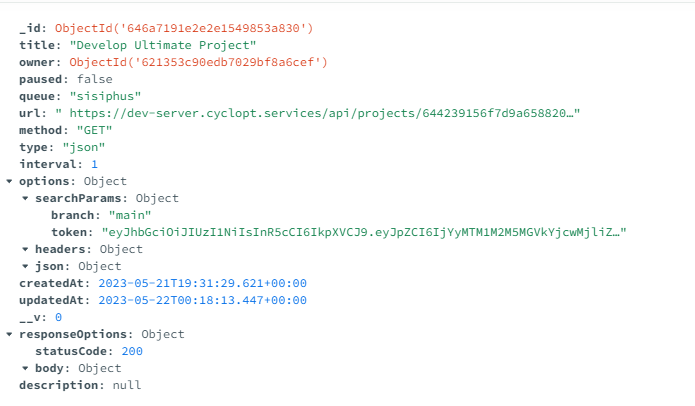
\includegraphics[width=0.8\textwidth]{./images/chapter4/api_doc.png}
			\caption[Παράδειγμα εγγραφής ενός \textbf{Api} στη βάση]{Παράδειγμα εγγραφής ενός \textbf{Api} στη βάση}
			\label{fig:api_doc}
		\end{figure}
	\item Για να γίνει όμως η αποθήκευση θα πρέπει πρώτα να ξεκινήσει ένα post αίτημα στον server του συστήματός μας, στο σώμα του οποίου
		θα περιέχονται όλες οι επιλογές που έχει κάνει ο χρήστης. Πριν, όμως, ο server το αποθηκεύσει στη βάση, ψάχνει τον πιο ελέυθερο, από 
		άποψη φόρτου, worker. Αυτό γίνεται μετρώντας τις καταχωρήσεις των collections που αντιστοιχούν σε κάθε έναν από αυτούς. Αφού εντοπιστεί 
		και επιλεχθεί ο καταλληλότερος, δημιουργεί ένα \textit{Api} αντικείμενο στη βάση δεδομένων καθώς και ένα \textit{job} στο collection του αντίστοιχου worker.
	\item Στη συνέχεια και για να ακολουθήσουμε τη ροή του συστήματος, μεταφερόμαστε στους workers και πιο συγκεκριμένα σε αυτόν που επιλέχθηκε
		στο προηγούμενο βήμα. H λειτουρία αυτού του τμήματος του Lychte μελετήθηκε παραπάνω. Αυτό το οποίο δεν αναφέραμε είναι το τι ακριβώς κάνει κάθε process
		που τρέχει εντός του worker. Κάθε τέτοιο child process, έχοντας ως δεδομένο ένα \textit{Api} αντικείμενο (αυτό που αποθηκεύτηκε σε προηγούμενο στάδιο από τον server)
		γνωρίζει που πρέπει να απευθύνεται το αίτημα που εκτελεί, καθώς και τις παραμέτρους που ίσως αυτό χρειάζεται. Επίσης είναι υπεύθυνο δυνητικά για το έλεγχο της
		ορθότητας της απόκρισης του εξωτερικού συστήματος, μέσα από την σύγκριση της με τα στοιχεία που έδωσε ο χρήστης κατά τη δημιουργία του Api, καθώς και για την ενημέρωση του χρήστη
		σε περίπτωση αποτυχίας του αιτήματος, μέσω email, εφόσον ο ίδιος το επιθυμεί. Αν 
		ανάλογη πληροφορία δεν υπάρχει αποθηκευμένη στη βάση, δεν πραγματοποιούνται έλεγχοι και η απάντηση που λαμβάνουμε αποθηκεύεται στη βάση δεδομένων. Αξίζει να σημειωθεί
		ότι όταν ο τύπος της απάντησης που επιστρέφεται είναι οποιοσδήποτε πέραν του json, δεν αποθηκεύεται
		το πραγματικό response, αλλά το αποτέλεσμα της απάντησης, αν δηλαδή εκτελέστηκε επιτυχώς ή όχι (συνεπώς αποθηκεύεται μία Boolean μεταβλητή).
		Πέρα από αυτά κρατάμε ακόμα τους χρονισμούς του αιτήματος (πότε ξεκίνησε, πότε ολοκληρώθηκε, πόσο διήρκησε) και δύο ακόμα Boolean μεταβλητές που σχετίζονται με σφάλματα που εμφανίστηκαν
		κατά την εκτέλεση του (σφάλμα είτε του δικού μας συστήματος είτε του εξωτερικού συστήματος).  
		\begin{figure}[!ht]
			\centering
			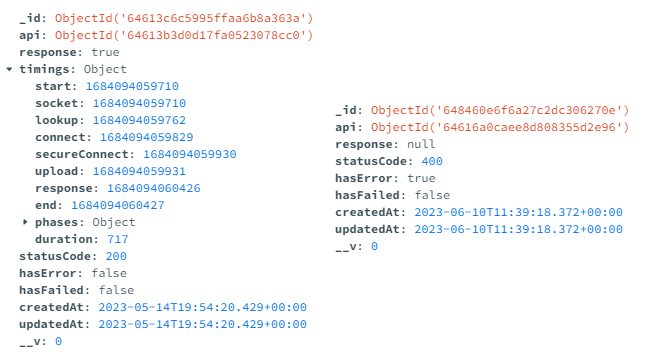
\includegraphics[width=0.8\textwidth]{./images/chapter4/response_docs.png}
			\caption[Παράδειγμα εγγραφών \textbf{Response} στη βάση]{Παράδειγμα εγγραφής \textbf{Response} στη βάση. Αριστερά βλέπουμε ένα επιτυχές response και δεξιά ένα που απέτυχε λόγω σφάλματος από τη μεριά του υπό παρακολούθηση συστήματος (το καταλαβαίνουμε από το πεδίο hasError που είναι true).}
			\label{fig:response_docs}
		\end{figure}
	\item Τέλος, η πληροφορία που αποθηκεύεται σε όλα τα στάδια της διαδικασίας στέλνεται στον client, κάθε φορά που αυτός, χρησιμοποιώντας τη γραφική διεπαφή
		που δημιουργήσαμε, επιλέγει να δει τα διάφορα διαγράμματα και μετρικές που υπολογίζουμε με τα δεδομένα που αφορούν το αίτημα που θέλει να ελέγξει.
\end{enumerate}

Το σύστημα όμως, όπως είναι τώρα, δεν είναι σε θέση να μπορεί να δείχνει επαρκώς γρήγορα ιστορικά δεδομένα. Αν υποθέσουμε ότι έχουμε ένα Api που θέλουμε να ελέγχουμε κάθε
λεπτό, στο τέλος της ημέρας θα έχουν μαζευτεί από αυτό και μόνο 1.440 εγγραφές. Αν αυτά συνεχίζουν να μαζεύονται, τότε ακόμα και τα πιο απλά queries στο μοντέλο των αποκρίσεων θα καθυστερούν, καθιστώντας έτσι την εφαρμογή λιγότερο ανταποκρίσιμη.
Για την αποφυγή συσσώρευσης περιττής, μετά από ορισμένο χρονικό διάστημα, πληροφορίας, έχουμε βάλει επιπρόσθετα σε κάθε worker ένα ακόμα job που αφορά
τον καθαρισμό της βάσης από εγγραφές που προέρχονται από το καθένα. Η διεργασία αυτή τρέχει μία φορά την εβδομάδα. Κάθε φορά που εκτελείται ψάχνει τα Apis ανάλογα με τον worker στον οποίο τρέχει.
Έπειτα μαζεύει όλες τις αποκρίσεις που σχετίζονται με το κάθε Api ξεχωριστά και ξεκινάει τους υπολογισμούς. Τα δεδομένα που αντλούνται στο πλαίσιο αυτής της διεργασίας στο τέλος διαγράφονται από τη βάση, ώστε ολα τα αιτήματα προς τη βάση
να εκτελούνται πιο γρήγορα και αποδοτικά. Σβήνοντας όμως πληροφορία, χάνουμε την ιστορικότητα των δεδομένων μας, με αποτέλεσμα να χάνουν και οι χρήστες μία πιο γενική εικόνα των ελέγχων που έχουν πραγματοποιηθεί.
Στο σημείο αυτό εισάγεται μία άλλης μορφής βάση δεδομένων, η Google Cloud Storage.

Πριν σβήσουμε δεδομένα που κρίνουμε ότι δεν έιναι απαραίτητο να υπάρχουν στη βάση, αλλά έχουν αξία για ιστορική ανάλυση, τα μεταφέρουμε στο Cloud Storage της Google, υπό μορφή αρχείων.
Με τον τρόπο αυτό κερδίζουμε χώρο, στη κεντρική Mongo βάση, στη λειτουργία της οποίας στηρίζεται όλο το σύστημα, και γενικά απόδοση καθώς έχει καλύτερες ταχύτητες στο σύνολο.

\begin{figure}[!ht]
	\centering
	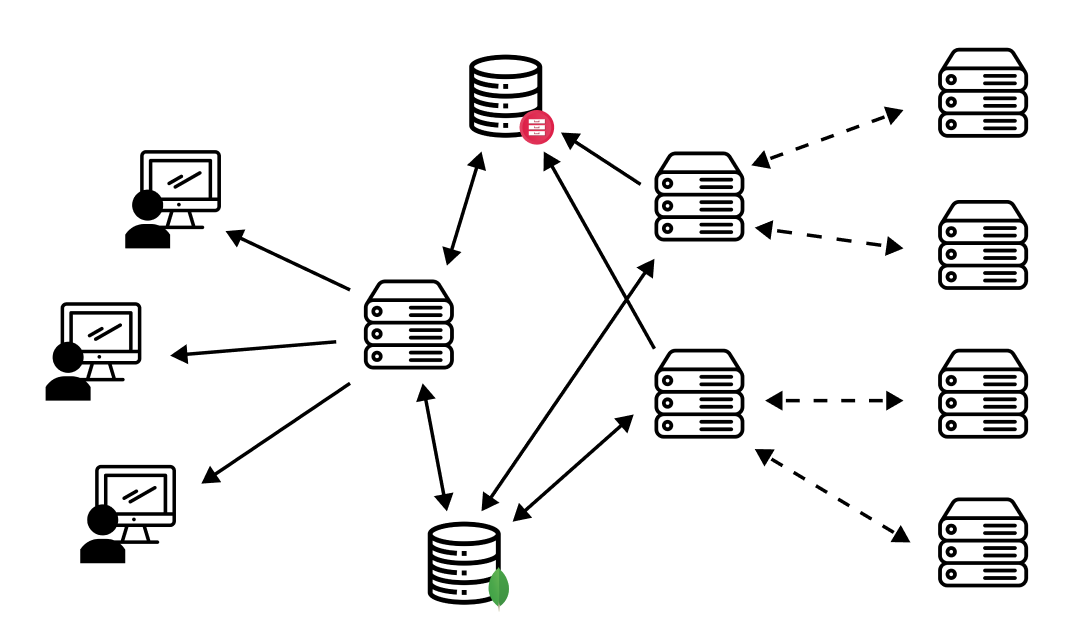
\includegraphics[width=0.8\textwidth]{./images/chapter4/lychte-third-implementation-full.png}
	\caption[Τελικό διάγραμμα Lychte]{Τελικό διάγραμμα Lychte}
	\label{fig:lychte_finalised}
\end{figure}


Πριν συνεχίσουμε στο κομμάτι των αποτελεσμάτων θα αναφερθούμε πιο συγκεκριμένα στις
ενέργειες που εκτελεί η παραπάνω διαδικασία:

\begin{enumerate}
	\item Συλλογή όλων το Responses που υπάρχουν αποθηκευμένα στη βάση, μέχρι μία μέρα πριν την εκτέλεση της διεργασίας καθαρισμού. Αυτό γίνεται προκειμένου να σιγουρευτούμε ότι υπάρχει πάντα πληροφορία στη βάση για την προηγούμενη ημέρα που μπορούμε να δείξουμε.
	\item Δημιουργία δύο διαφορετικών πινάκων, ενός που αποθηκεύει του χρόνους διάρκειας των αιτημάτων και ενός που περιέχει Boolean μεταβλητές σχετικά με το αν τα αιτήματα γίνονται επιτυχώς ή όχι.
	\item Στη συνέχεια, για κάθε μέρα στην οποία έχουμε εγγραφές Responses, υπολογίζουμε και αποθηκεύουμε στατιστικά σχετικά με τη μέση τιμή, διάμεσο και τυπική απόκλιση διάρκειας αιτημάτων.
	\item Στο τέλος της διαδικασίας αποθηκεύονται τρία αρχεία για κάθε Api. Ένα στο οποίο περιέχονται τα responses όπως ακριβώς ήταν αποθηκευμένα στη mongodb (σε αρχείο της μορφής \textbf{"../apiId/raw-responses/MM-DD-YYYY.json"}),
		ένα που περιέχει τους πίνακες που περιγράψαμε στο δεύτερο βήμα (\textbf{"../apiId/\hyp{}raw-values/MM-DD-YYYY.avro"}) και τέλος, ένα αρχείο που περιέχει κάποια χρήσιμα στατιστικά για κάθε μέρα που εντοπίστηκε, όπως περιγράφεται στο βήμα τρία (\textbf{"../apiId/statistics.avro"}) 
\end{enumerate}

Επειδή τα αρχεία που περιέχουν στατιστικά για κάθε μέρα χρησιμοποιούνται αρκετά συχνά από τη γραφική διεπαφή του Lychte για την παρουσίαση ιστορικών δεδομένων του υπό μελέτη Api, κρίναμε απαραίτητη τη χρήση ενός διαφορετικού τύπου αρχείου σε σχέση με
τον κλασσικό και ευρέως διαδεδομένο στο διαδίκτυο τύπο JSON, το AVRO, για να κερδίσουμε ως προς τον αποθηκευτικό χώρο αλλά και την ταχύτητα ανάγνωσης. Αξίζει να σημειωθεί ότι ένα αρχέιο avro σε σχέση με ένα αρχείο json που περιέχουν ακριβώς την ίδια
πληροφορία, για τα στατιστικά στα οποία αναφερόμαστε, είναι 70\% περίπου μικρότερο σε μέγεθος (json αρχείο 250Μb, avro αρχείο 75Μb)
Ο λόγος που μπορούμε να χρησιμοποιήσουμε avro αρχεία είναι ότι η μορφή της αποθηκευμένης πληροφορία παραμένει ίδια και δεν αλλάζει. Πιο συγκεκριμένα, τα schemas που χρησιμοποιούνται στα αρχεία \textbf{"raw-values/MM-DD-YYYY.avro"} και \textbf{"statistics.avro"}
φαίνονται στο \autoref{fig:avro_types}.

\begin{figure}[!ht]
	\centering
	\makebox[\textwidth][c]{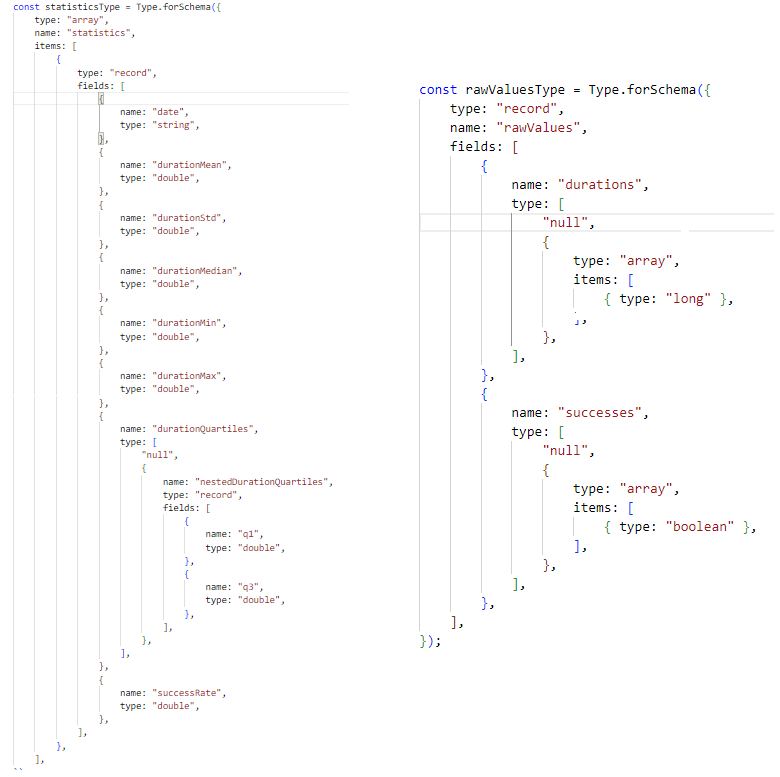
\includegraphics[width=1\textwidth]{./images/chapter4/avro_types.png}}
	\caption[Schemas πληροφορίας που αποθηκεύουμε σε avro αρχεία]{Schemas πληροφορίας που αποθηκεύουμε σε avro αρχεία. Το πρώτο αφορά τα statistics που αποθηκεύονται και αποτελείται από ένα array από objects, τα fields των οποίων σχετίζονται σε μετρικές στατιστικής φύσης. Το δεύτερο schema χαρακτηρίζει τα raw-values που αποθηκεύουμε και αποτελείται από ένα object με δύο arrays}
	\label{fig:avro_types}
\end{figure}

